\begin{enunciado}
 En el ejercicio 1.18 de la p\'agina 28, pruebe la bondad de ajuste
 entre las frecuencias de clase que se observan,
 y las frecuencias esperadas correspondientes de una distribuci\'on normal
 con $\mu = 65$ y $\sigma = 21$.
 Utilice un nivel de significancia de $0.05$.
\end{enunciado}

\begin{solucion}
 La resoluci\'on se har\'a usando ambas pruebas vistas en el libro:
 la prueba de bondad de ajuste $\chi^2$ y la prueba de Geary.
 \begin{datos}
  Usando los datos del ejercicio 1.18, incluyendo el diagrama de tallo y hoja, 
  se tiene lo siguiente:
  \begin{itemize}
   \item Tama\~no de la muestra: $n=60$.
   \item Media muestral: $\bar{x} = \frac{3\,929}{60} = 65.38\bar{3}$.
   \item Varianza muestral:
   $s^2 = \frac{1\,581\,059}{3\,540} \approx 44.6776836158192$
   \item Frecuencia observada individualmente:
   \begin{center}
    \begin{tabular}{ccccccccc}
     $23$ & $60$ & $79$ & $32$ & $57$ & $74$ & $52$ & $70$ & $82$ \\
     $36$ & $80$ & $77$ & $81$ & $95$ & $41$ & $65$ & $92$ & $85$ \\
     $55$ & $76$ & $52$ & $10$ & $64$ & $75$ & $78$ & $25$ & $80$ \\
     $98$ & $81$ & $67$ & $41$ & $71$ & $83$ & $54$ & $64$ & $72$ \\
     $88$ & $62$ & $74$ & $43$ & $60$ & $78$ & $89$ & $76$ & $84$ \\
     $48$ & $84$ & $90$ & $15$ & $79$ & $34$ & $67$ & $17$ & $82$ \\
     $69$ & $74$ & $63$ & $80$ & $85$ & $61$
    \end{tabular}
   \end{center}
   las cuales se pueden agrupar en las $9$ clases que hicieron
   en el diagrama de tallo y hoja del ejercicio al que se hace referencia, 
   lo cual se muestra en la siguiente tabla:
   \begin{center}
    \begin{tabular}{cc}
     \hline 
     \textbf{L\'{\i}mites de clase} & $o_i$ \\
     \hline 
     $ 9.5 - 19.5$ &  $3$ \\
     $19.5 - 29.5$ &  $2$ \\
     $29.5 - 39.5$ &  $3$ \\
     $39.5 - 49.5$ &  $4$ \\
     $49.5 - 59.5$ &  $5$ \\
     $59.5 - 69.5$ & $11$ \\
     $69.5 - 79.5$ & $14$ \\
     $79.5 - 89.5$ & $14$ \\
     $89.5 - 99.5$ &  $4$ \\
     \hline 
    \end{tabular}
   \end{center}
   \item Probabilidades esperadas: usando la tabla A.3,
   se encuentra las \'areas bajo la curva para cada clase como sigue:
   \begin{center}
    \begin{tabular}{cccc}
     \hline 
     \multicolumn{3}{c}{\textbf{L\'{\i}mites de clase}} & $p_i$ \\
     \hline 
     $ 9.5$ & $-$ & $19.5$ &
     $P\left( Z<\frac{19.5 - 65}{21}\right) \approx P(Z<-2.17)\approx 0.0150$ \\
     $19.5$ & $-$ & $29.5$ &
     $P\left( \frac{19.5 - 65}{21} < Z < \frac{29.5 - 65}{21} \right)
     \approx P(Z < -1.69) - P(Z < -2.17)$ \\
     & & & $\approx 0.0455 - 0.0150 = 0.0305$ \\
     $29.5$ & $-$ & $39.5$ &
     $P\left( \frac{29.5 - 65}{21} < Z < \frac{39.5 - 65}{21} \right)
     \approx P(Z < -1.21) - P(Z < -1.69)$ \\
     & & & $\approx 0.1131 - 0.0455 = 0.0676$ \\
     $39.5$ & $-$ & $49.5$ &
     $P\left( \frac{39.5 - 65}{21} < Z < \frac{49.5 - 65}{21} \right)
     \approx P(Z < -0.74) - P(Z < -1.12)$ \\
     & & & $\approx 0.2296 - 0.1131 = 0.1165$ \\
     $49.5$ & $-$ & $59.5$ &
     $P\left( \frac{49.5 - 65}{21} < Z < \frac{59.5 - 65}{21} \right)
     \approx P(Z < -0.26) - P(Z < -0.74)$ \\
     & & & $\approx 0.3974 - 0.2296 = 0.1678$ \\
     $59.5$ & $-$ & $69.5$ &
     $P\left( \frac{59.5 - 65}{21} < Z < \frac{69.5 - 65}{21} \right)
     \approx P(Z < 0.21) - P(Z < -0.26)$ \\
     & & & $\approx 0.5832 - 0.3974 = 0.1858$ \\
     $69.5$ & $-$ & $79.5$ &
     $P\left( \frac{69.5 - 65}{21} < Z < \frac{79.5 - 65}{21} \right)
     \approx P(Z < 0.69) - P(Z < 0.21)$ \\
     & & & $\approx 0.7549 - 0.5832 = 0.1717$ \\
     $79.5$ & $-$ & $89.5$ &
     $P\left( \frac{79.5 - 65}{21} < Z < \frac{89.5 - 65}{21} \right)
     \approx P(Z < 1.17) - P(Z < 0.69)$ \\
     & & & $\approx 0.879 - 0.7549 = 0.1241$ \\
     $89.5$ & $-$ & $99.5$ &
     $P\left( \frac{89.5-65}{21}<Z\right)\approx 1-P(Z < 1.17)\approx 1 - 0.879 = 0.121$ \\
     \hline
    \end{tabular}
   \end{center}
   \item Frecuencias esperadas, determinado por clase
   y considerando el redondeo a un decimal: $E = \left\{
   \left.e_i=n\cdot p_i\,\right|\,\forall i\in\mathbb{N}\cap[1,9] \right\}
   = \{ e_1 = 60\times 0.015 = 0.9, e_2 = 60 \times 0.0305 = 1.8,
   e_3 = 60 \times 0.0676 = 4.1, e_4 = 60 \times 0.1165 = 7,
   e_5 = 60 \times 0.1678 = 10.1, e_6 = 60 \times 0.1858 = 11.1,
   e_7 = 60 \times 0.1717 = 10.3, e_8 = 60 \times 0.1241 = 7.4,
   e_9 = 60 \times 0.121 = 7.3 \}$
  \end{itemize}
  Dado que las pruebas de bondad por m\'etodo de $\chi^2$ no son confiables
  cuando la frecuencia esperada de una celda es menor a $5$,
  se agrupar\'an los datos, como sigue:
  \begin{itemize}
   \item Frecuencias observadas, probabilidades esperadas y frecuencias
   esperadas por clase, se muestran a continuaci\'on en la siguiente tabla:
   \begin{center}
    \begin{tabular}{ccccccc}
     \hline
     \textbf{L\'{\i}mites de clase} & $o_i$ & & $p_i$ & & $e_i$ & \\
     \hline 
     $ 9.5 - 19.5$ &  $3$ &
     \multirow{3}{*}{\hspace{-0.7cm} $\left.
     \begin{matrix}\phantom{0}\\\phantom{0}\\\phantom{0}\end{matrix}
     \right\} 8$}
     & $0.015$ &
     \multirow{3}{*}{\hspace{-0.5cm}$\left.
     \begin{matrix}\phantom{0}\\\phantom{0}\\\phantom{0}\end{matrix}
     \right\} 0.1131$}
     & $0.9$ &
     \multirow{3}{*}{\hspace{-0.7cm} $\left.
     \begin{matrix}\phantom{0}\\\phantom{0}\\\phantom{0}\end{matrix}
     \right\} 6.8$} \\
     $19.5 - 29.5$ &  $2$ &\hspace{-0.7cm}& $0.0305$ &\hspace{-0.5cm}& $1.8$  \\
     $29.5 - 39.5$ &  $3$ &\hspace{-0.7cm}& $0.0676$ &\hspace{-0.5cm}& $4.1$  \\
     $39.5 - 49.5$ &  $4$ &\hspace{-0.7cm}& $0.1165$ &\hspace{-0.5cm}&  $7$   \\
     $49.5 - 59.5$ &  $5$ &\hspace{-0.7cm}& $0.1678$ &\hspace{-0.5cm}& $10.1$ \\
     $59.5 - 69.5$ & $11$ &\hspace{-0.7cm}& $0.1858$ &\hspace{-0.5cm}& $11.1$ \\
     $69.5 - 79.5$ & $14$ &\hspace{-0.7cm}& $0.1717$ &\hspace{-0.5cm}& $10.3$ \\
     $79.5 - 89.5$ & $14$ &\hspace{-0.7cm}& $0.1241$ &\hspace{-0.5cm}& $7.4$  \\
     $89.5 - 99.5$ &  $4$ &\hspace{-0.7cm}&  $0.121$ &\hspace{-0.5cm}& $7.3$  \\
     \hline 
    \end{tabular}
   \end{center}
   \item Celdas totales del experimento: $k=7$.
   \item Grados de libertad de la prueba $\chi^2$: $v= k-1 = 6$.
  \end{itemize}
 \end{datos}
 
 \begin{hipotesis}
  Prueba de bondad de ajuste para probar $H_0:$
  que la variable aleatoria $X$, de la calificaci\'on en el examen final
  para el curso de estad\'{\i}stica elemental,
  sigue una distribuci\'on normal
  con media $\mu=6.5$ y desviaci\'on est\'andar $\sigma = 2.1$,
  contra la alternativa $H_1$ de que no es as\'{\i}.
 \end{hipotesis}

 \begin{significancia}
  $\alpha = 0.05$.
 \end{significancia}

 \begin{region}
  De la tabla A.5, se tiene el valor cr\'{\i}tico
  $\chi^2_{\alpha,v} = \chi^2_{0.05,6} \approx 12.592$,
  por lo que la regi\'on de rechazo est\'a dado
  para $\chi^2 > 12.592$, donde
  $\chi^2 = \sum_{i=1}^{k} \frac{\left( o_i - e_i \right)^2}{e_i}$.
  O bien, de la tabla A.3, se tiene el valor cr\'{\i}tico
  $Z_{\alpha/2} = Z_{0.025} \approx 1.96$,
  por lo que la regi\'on de rechazo tambi\'en est\'a dado
  para $Z < -1.96$ o $Z > 1.96$,
  donde $Z = \frac{U - 1}{0.2661/\sqrt{n}}$ y, a su vez,
  $U = \frac{\sqrt{\pi/2} \sum_{i=1}^{n} \left| X_i - \overline{X} \right|/n}{
  \sqrt{\sum_{i=1}^n \left( X_i - \overline{X} \right)^2/n}}$
 \end{region}

 \begin{estadistico}
  Para la prueba de $\chi^2$, el estad\'{\i}stico est\'a dado por:
  \begin{eqnarray*}
   \chi^2 & = & \sum_{i=1}^{k} \frac{\left( o_i - e_i \right)^2}{e_i} \\
   & \approx & \frac{(8-6.8)^2}{6.8} + \frac{(4-7)^2}{7} +
   \frac{(5-10.1)^2}{10.1} + \frac{(11-11.1)^2}{11.1} + \\
   & & 
   \frac{(14-10.3)^2}{10.3} + \frac{(14-7.4)^2}{7.4} + \frac{(4-7.3)^2}{7.3} \\
   & = & \frac{1.44}{6.8} + \frac{9}{7} + \frac{26.01}{10.1} +
   \frac{0.01}{11.1}+\frac{13.69}{10.3}+\frac{43.56}{7.4}+\frac{10.89}{7.3} \\
   & \approx & 0.2118 + 1.2857 + 2.5752 + 0.0009 + 1.3291 + 5.8865 + 1.4918
   = 12.781
  \end{eqnarray*}
  Mientras que, para la prueba de Geary, el c\'alculo del estad\'{\i}stico
  se realiza como sigue, realizando previamente algunos c\'alculos:
  \par 
  Primero se requieren los valores de $x_i - \bar{x}$, los cuales se
  han calculado en el proceso de obtener la desviaci\'on est\'andar
  durante la soluci\'on del problema 1.18, luego entonces, se tiene que:
  \begin{eqnarray*}
   \sum_{i=1}^{60} \left| x_i - \overline{x} \right| & = &
   \frac{1}{60}\left( |-2549| + |-329| + |811| + |-2009| + |-509| + |511| +
   |-809| + |271| + \right. \\
   & & \phantom{\frac{1}{60}(} |991| + |-1769| + |871| + |691| + |931| +
   |1771| + |-1469| + |-29| + \\
   & & \phantom{\frac{1}{60}(} |1591| + |1171| + |-629| + |631| + |-809| +
   |-3329| + |-89| + |571| + \\
   & & \phantom{\frac{1}{60}(} |751| + |-2429| +  |871| + |1951| + |931| + 
   |91| + |-1469| + |331| +  |1051| + \\
   & & \phantom{\frac{1}{60}(} |-689| + |-89| + |391| + |1351| + 
   |-209| + |511| + |-1349| + |-329| + \\
   & & \phantom{\frac{1}{60}(} |751| + |1411| + |631| + |1111| + |-1049| + 
   |1111| + |1471| + |-3029| + \\
   & & \phantom{\frac{1}{60}(} |811| + |-1889| + |91| + |-2909| + |991| + 
   |211| + |511| + |-149| + |871| + \\
   & & \phantom{\frac{1}{60}(} \left. |1171| + |-269| \right)
   = \frac{60\,370}{60} = \frac{6\,037}{6} = 1\,006.1\bar{6}
  \end{eqnarray*}
  y
  \begin{equation*}
   \sum_{i=1}^{60} \left( x_i - \overline{x} \right)^2 = s^2\times 59 =
   \frac{1\,581\,059}{3\,540} \times 59 = \frac{1\,581\,059}{60}
  \end{equation*}
  Luego entonces
  \begin{eqnarray*}
   U & = & \frac{
   \displaystyle{\sqrt{\pi/2}
   \frac{\sum_{i=1}^n \left| X_i - \overline{X} \right|}{n}}
   }{
   \displaystyle{\sqrt{
   \frac{\sum_{i =1}^n \left( X_i - \overline{X} \right)^2}{n}}}
   } 
   = \frac{\displaystyle{\sqrt{\pi/2} \frac{6\,037}{360}}}{
   \displaystyle{\sqrt{ \frac{1\,581\,059}{3\,600} }}}
   = \frac{\displaystyle{\sqrt{\pi} \frac{6\,037}{\cancelto{6}{360}}}}{
   \displaystyle{ \frac{\sqrt{2 \times 1\,581\,059}}{\cancel{60}} }}
   = \frac{\sqrt{3\,162\,118\pi} 6\,037}{3\,162\,118\times 6} \\
   & = & \frac{6\,037\sqrt{3\,162\,118\pi}}{18\,972\,708}
   \approx 1.00289583
  \end{eqnarray*}
  Por lo que el estad\'{\i}stico $Z$ para la prueba de Geary es:
  \begin{eqnarray*}
   Z & = & \frac{U - 1}{0.2661/\sqrt{n}} = 
   \frac{\displaystyle{\frac{6\,037\sqrt{3\,162\,118\pi}}{18\,972\,708} - 1}
   }{\displaystyle{\frac{0.2661}{\sqrt{60}}}}
   = \frac{\displaystyle{
   \frac{6\,037\sqrt{3\,162\,118\pi} - 18\,972\,708}{18\,972\,708}}}{
   \displaystyle{\frac{2\,661}{10\,000\cdot 2\sqrt{15}}}} \\
   & = & \frac{\cancelto{5\,00}{20\,000}\,\,\,\sqrt{15} \cdot
   \left(6\,037\sqrt{3\,162\,118\pi} - 18\,972\,708\right)}{
   2\,661\cdot \cancelto{4\,743\,177}{18\,972\,708}} \\
   & = & \frac{5\,000\sqrt{15}\left(
   6\,037\sqrt{3\,162\,118\pi}-18\,972\,708\right)}{
   12\,621\,593\,997} \approx 0.084295 \\
  \end{eqnarray*}
 \end{estadistico}

 \begin{decision}
  Se presenta una discrepancia al comparar las pruebas de bondad de $\chi^2$
  y de Geary.
  En la literatura se sugiere que, si existe discrepancia entre dos pruebas,
  se debe tomar una decisi\'on conservadora, es decir,
  se rechaza $H_0$ a favor de $H_1$.
 \end{decision}

 \begin{conclusion}
  Se obtiene evidencia suficiente, por la prueba $\chi^2$, para afirmar
  que las calificaciones en el examen final del curso de estad\'{\i}stica
  elemental no sigue una distribuci\'on normal con media $\mu = 6.5$
  y desviaci\'on est\'andar $\sigma = 2.1$.
 \end{conclusion}
 
 En el c\'odigo registrado en el archivo
 \texttt{P17\_Prueba\_de\_normalidad\_01.r} se realiza este procedimiento.
 El c\'odigo permite modificar los valores iniciales que corresponden a:
 \texttt{datos} que guarda los datos de la lectura de un archivo,
 en este caso se lee el archivo \texttt{BD24\_Problema\_088.csv},
 y este \'ultimo nombre es el que se modifica para leer otros archivos;
 \texttt{varInteres} para indicar el nombre de la columna
 que corresponde a los datos;
 \texttt{media} y \texttt{desv.est} para indicar valores presupuestos
 para la media y la desviaci\'on est\'andar,
 o bien se les puede asignar \texttt{NULL} y se
 estimar\'an los valores;
 \texttt{clases} para indicar con un n\'umero la cantidad de clases
 a considerar o una lista con los n\'umeros m\'aximos y m\'{\i}nimo
 de todas las clases, as\'{\i} como tambi\'en los valores de corte
 que separan cada clase,
 o bien indicar con \texttt{NULL} si se desee crear la divisi\'on de clases
 de forma autom\'atica;
 y \texttt{graficaHist} para indicar, con \texttt{TRUE},
 si se desea realizar una gr\'afica de comparaci\'on entre la distribuci\'on
 normal supuesta y la distribuci\'on de la muestra en un histograma,
 o \texttt{FALSE} en caso contrario.
 \par
 El programa espera al menos los datos correspondientes a la base de datos,
 escrito en un arhivo \texttt{.csv} con una columna con los datos, 
 identificado por \texttt{varInteres}.
 \par
 El programa realiza los c\'alculos de bondad de ajuste correspondientes
 a los m\'etodos vistos en el libro, es decir, por el m\'etodo $\chi^2$,
 considerado tambi\'en como m\'etodo de Pearson,
 y el m\'etodo de Geary.
 Adem\'as de estos m\'etodos, se calculas los estad\'{\i}sticos
 correspondientes a las pruebas de Kolmogorov-Smirnov, el de Lilliefors,
 que es una versi\'on mejorada del de Kolmogorov-Smirnov (K-S)
 para las pruebas de normalidad y el de Shapiro-Wilk.
 Adem\'as de los estad\'{\i}sticos, se calculan los $p-$valores de estos.
 Aunque tienen sus respectivas diferencias, se hace notar aqu\'{\i}
 algunas de ellas:
 el m\'etodo $\chi^2$ y el de Kolmogorov-Smirnov son los \'unicos
 m\'etodos que usan las supociones de los par\'amtros poblaciones hechas mientras que el resto de m\'etodos usan siempre estimaciones
 a partir de los datos independientemente de que existan supociones previas;
 por otro lado, los m\'etodos de bondad de ajuste $\chi^2$ y K-S
 son gen\'ericos, mientras que el resto sirven para pruebas de normalidad
 en espec\'{\i}fico.
 Cabe hacer notar que en este programa no se indicar\'an regiones de rechazo, 
 ya que no se encuentran en algunos de estos m\'etodos los procesos inversos
 para calcular una regi\'on de rechazo a partir de un valor de probabilidad.
 Finalmente, cabe mencionar que se usar\'an los paquetes \texttt{MASS}
 y \texttt{nortest} para los gr\'aficos y para la prueba de Lilliefors,
 respectivamente.
 \par
 El programa siempre mostrar\'a en su salida lo siguiente:
 \texttt{nombres} que contiene el nombre de la variable de los datos;
 \texttt{n} para el tama\~no muestral usado;
 \texttt{X de chi2} que indica el estad\'{\i}stico $\chi^2$
 del m\'etodo $\chi^2$ de Pearson;
 \texttt{param chi2} que indica la cantidad de grados de libertad
 usado durante el m\'etodo de $\chi^2$;
 \texttt{Valor-p chi2} para indicar el $p-$valor calculado
 durante el m\'etodo de $\chi^2$;
 \texttt{Z de Geary} con el valor del estad\'{\i}stico $Z$
 calculado con la prueba de Geary;
 \texttt{Valor-p Geary} para indicar el $p-$valor calculado
 durante la prueba de Geary;
 \texttt{D de K-S} con el valor del estad\'{\i}stico $D$
 calculado con la prueba de Kolmogorov-Smirnov;
 \texttt{Valor-p K-S} para indicar el $p-$valor calculado
 con el estad\'{\i}stico $D$ de Kolmogorov-Smirnov;
 \texttt{D de K-S Lilliefors} con el valor del estad\'{\i}stico $D$
 calculado con la prueba de Lilliefors-Kolmogorov-Smirnov;
 \texttt{Valor-p K-S Lilliefors} para indicar el $p-$valor calculado
 con el estad\'{\i}stico $D$ de Lilliefors-Kolmogorov-Smirnov;
 \texttt{W de Shapiro} con el valor del estad\'{\i}stico $W$
 calculado con la prueba de Shapiro-Wilk;
 y, finalmente, \texttt{valor-p Shapiro} para indicar el $p-$valor calculado
 durante la prueba de Shapiro-Wilk.
 El c\'odigo junto con el resultado se muestra a continuaci\'on:
 \begin{verbatim}
> require(MASS)
> require(nortest)
> datos<-read.csv("DB24_Problema_088.csv",sep=";",encoding="UTF-8")
> varInteres<-"Calificación"
> media<-65
> desv.est<-21
> clases<-c(9.5,19.5,29.5,39.5,49.5,59.5,69.5,79.5,89.5,99.5)
> graficaHist<-TRUE
> colapsar<-function(p1,f1,lim1=5){
+   np1<-p1
+   nf1<-f1
+   tocollapse<-which((p1*sum(f1))<lim1)
+   while(length(tocollapse)>0){
+     x<-tocollapse[1]
+     if (x<(length(f1)/2)){
+       np1[x+1]<-p1[x]+p1[x+1]
+       nf1[x+1]<-f1[x]+f1[x+1]
+     }else{
+       np1[x-1]<-p1[x]+p1[x-1]
+       nf1[x-1]<-f1[x]+f1[x-1]
+     }
+     p1<-np1[-x]
+     f1<-nf1[-x]
+     np1<-p1
+     nf1<-f1
+     tocollapse<-which((p1*sum(f1))<lim1)
+   }
+   return(list(probs=p1,freqs=f1))  
+ }
> calculos2<-function(x,media=NULL,desv.est=NULL,clases){
+   n<-length(x)
+   ajuste<-0
+   if (is.null(media)) {
+     media<-mean(x)
+     ajuste<-ajuste+1
+   }
+   if (is.null(desv.est)) {
+     desv.est<-sd(x)
+     ajuste<-ajuste+1
+   }
+   if(is.null(clases)){
+     k<-round(sqrt(length(x)),0)
+     clases<-min(x)
+     clases<-c(clases,diff(range(x))/k*(1:(k-1))+min(x))
+     clases<-c(clases,max(x))
+   }
+   if(length(clases)==1){
+     k<-clases[1]
+     clases<-min(x)
+     clases<-c(clases,diff(range(x))/k*(1:(k-1))+min(x))
+     clases<-c(clases,max(x))
+   }
+   k<-length(clases)
+   frecObs<-hist(x,clases)$count
+   probEsp<-pnorm(clases[2],media,desv.est)
+   if(k>3) for(i in (2:(k-2))) {
+     probEsp<-c(probEsp,
+                pnorm(clases[i+1],media,desv.est,lower.tail=TRUE)
+                -pnorm(clases[i],media,desv.est,lower.tail=TRUE))
+   }
+   probEsp<-c(probEsp,1-sum(probEsp))
+   U<-sqrt(pi/2)*mean(abs(x-mean(x)))/sqrt(var(x)*(n-1)/n)
+   Geary.statistic<-(U-1)/(0.2661/sqrt(n))
+   Geary.p.value<-2*pnorm(abs(Geary.statistic),lower.tail=FALSE)
+   pruebaKSlillie<-lillie.test(x)
+   pruebaSW<-shapiro.test(x)
+   pruebaks<-ks.test(x[!duplicated(x)],"pnorm",mean=media,sd=desv.est)
+   ajuste<-0
+   r1<-colapsar(probEsp,frecObs)
+   frecObsC<-r1$freqs
+   probEspC<-r1$probs
+   if(length(frecObsC)>1){
+     pruebachisq<-chisq.test(frecObsC,p=probEspC)
+   }else{
+     pruebachisq<-NA
+   }
+   r<-c(n, pruebachisq$statistic, pruebachisq$parameter-ajuste,
+        pruebachisq$p.value, Geary.statistic, Geary.p.value,
+        pruebaks$statistic, pruebaks$p.value, pruebaKSlillie$statistic,
+        pruebaKSlillie$p.value, pruebaSW$statistic, pruebaSW$p.value)
+   return(r)
+ } 
> generaGrafica<-function(x,media,desv.est,clases,nombres){
+   if (is.null(media)) {
+     media<-mean(x)
+   }
+   if (is.null(desv.est)) {
+     desv.est<-sd(x)
+   }
+   if(is.null(clases)){
+     ni<-round(sqrt(length(x)),0)
+   }else if(length(clases)==1){
+     ni<-clases[1]
+   } else ni<-length(clases)
+   x11()
+   truehist(x,nbins=ni,sub=nombres,xlab="")
+   x<-seq(min(x)*.8,max(x)*1.2,l=100)
+   lines(x,dnorm(x,mean=media,sd=desv.est),lwd=1.5)
+ }
> valores<-datos[,varInteres]
> valores<-valores[!is.na(valores)]
> if(length(valores)<3){
+   stop("Se necesita de al menos 3 valores para proceder")
+ }
> r1<-t(as.matrix(calculos2(valores,media,desv.est,clases)))
> r1<-data.frame(nombre=varInteres,r1)
> names(r1)<-c("nombres","n","X de chi2", "param chi2", "Valor-p chi2",
+              "Z de Geary", "Valor-p Geary", "D de K-S", "Valor-p K-S",
+              "D de K-S Lilliefors", "Valor-p K-S Lilliefors",
+              "W de Shapiro","Valor-p Shapiro")
> r1
       nombres  n X de chi2 param chi2 Valor-p chi2 Z de Geary Valor-p Geary
1 Calificación 60  12.86244          6   0.04527318 0.08429539     0.9328216
    D de K-S Valor-p K-S D de K-S Lilliefors Valor-p K-S Lilliefors W de Shapiro
1 0.09817138   0.7534067           0.1398566            0.005196948    0.9176965
  Valor-p Shapiro
1    0.0006202501
> if (graficaHist){
+   generaGrafica(valores,media,desv.est,clases,varInteres)
+ }
 \end{verbatim}
 \vspace{-0.5cm}
 que incluye la siguiente figura:
 \begin{center}
  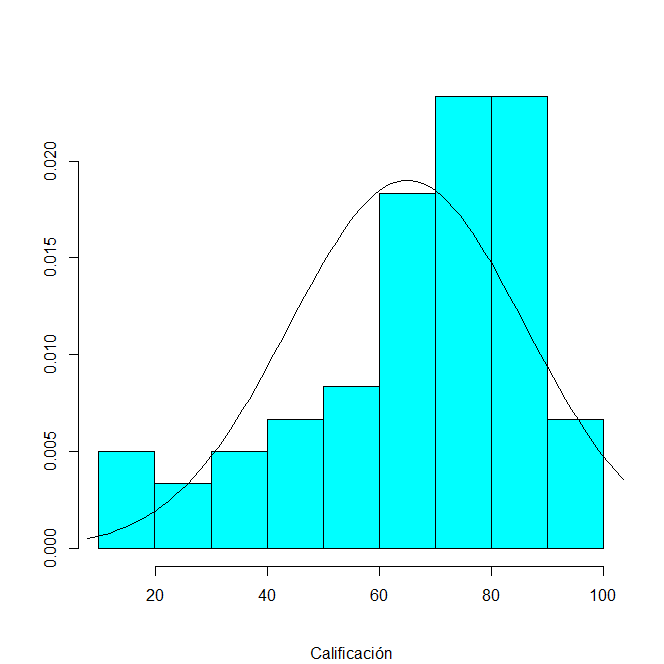
\includegraphics[scale=0.35]{Problema_88.png}
 \end{center}
 Lo cual coincide con los obtenido en las pruebas $\chi^2$ y de Geary.
 En el caso de la prueba $\chi^2$ hay una ligera discrepancia
 debido a los redondeos a un decimal.
 Adem\'as, se pueden observar c\'omo se obtiene valores de otras pruebas.
 En el caso de las pruebas K-S y Lilliefors, se requiere que no haya valores
 duplicados, por lo que podr\'{\i}a dudarse de su resultado,
 adem\'as de que su uso es recomendable para muestras grandes, mayores a $100$;
 por otro lado, la prueba de Shapiro-Wilk es bueno para meustras peque\~nas
 aunque sus ajuste es a par\'ametros estimados $\bar{x}$ y $s^2$.
 Luego entonces, se toma mayor fuerza en la prueba $\chi^2$,
 la cual ya indica que no hay un buen ajuste a una poblaci\'on normal,
 que es a lo que se quer\'{\i}a llegar.${}_{\blacksquare}$
\end{solucion}
